\section{ROS} \label{sec:ros}
ROS, cuyas siglas significan Robot Operating System, es un framework de software ampliamente utilizado en el desarrollo de aplicaciones robóticas. Aunque se le llama “sistema operativo”, ROS en realidad no es un sistema operativo completo como Windows o Linux, sino un conjunto de bibliotecas, herramientas y convenciones diseñadas para facilitar la creación de software para robots.


ROS proporciona una infraestructura flexible que permite a los desarrolladores crear sistemas robóticos complejos de forma modular, escalable y colaborativa. Esto se logra mediante la creación de nodos independientes que se comunican entre sí a través de un sistema de mensajes. Cada nodo puede encargarse de tareas específicas, como leer sensores, controlar motores, planear trayectorias o tomar decisiones, y todos estos módulos pueden intercambiar información de forma sincronizada en tiempo real. 
\cite{lovtechnology2024}


\begin{figure}[h]
	\centering
	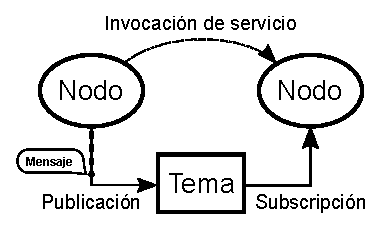
\includegraphics[width=0.5\linewidth]{img/ROS_concepts}
	\caption{Diagrama de comunicación de ROS}
	\label{fig:rosconcepts}
\end{figure}

Uno de los aspectos más importantes de ROS es su capacidad para abstraer la complejidad del hardware, lo que significa que los programadores pueden centrarse en la lógica y el comportamiento del robot sin preocuparse directamente por los detalles técnicos de cada componente físico. Gracias a esto, ROS ha sido adoptado en todo el mundo tanto en entornos académicos como industriales, y ha impulsado el desarrollo de robots móviles, brazos manipuladores, drones, vehículos autónomos, entre muchos otros. \cite{roboticsbackend2024}


\subsection{Nodo (Node)}

En el contexto de ROS (Robot Operating System), un nodo representa una unidad ejecutable que realiza una tarea específica dentro del sistema robótico. ROS está diseñado como un sistema distribuido, lo que significa que las tareas no se ejecutan en un único programa grande, sino que se dividen en varios nodos que pueden operar de forma independiente pero cooperativa. Por ejemplo, un nodo puede encargarse de leer datos de un sensor, otro puede controlar un motor, y un tercero puede realizar cálculos para la planificación de trayectorias. Esta arquitectura modular permite el desarrollo más organizado, reutilizable y escalable. Además, los nodos pueden ejecutarse en diferentes dispositivos conectados en red, lo que hace posible distribuir el procesamiento entre varios sistemas físicos. \cite{rosnode2024} 

\subsection{Tema (Topic)}
En ROS (Robot Operating System), un tópico es un canal de comunicación utilizado para el intercambio de mensajes entre nodos de forma asíncrona. A través de este mecanismo, un nodo puede publicar datos que otros nodos pueden recibir si están suscritos al mismo canal, sin necesidad de que haya una conexión directa entre ellos. Esto permite una arquitectura flexible y modular en la que distintos componentes del sistema pueden operar de manera independiente, facilitando el desarrollo y la escalabilidad de los proyectos. 

Por ejemplo, un nodo que lee datos de un sensor LiDAR puede publicar esa información constantemente en un tópico llamado "scan", mientras otros nodos, como los encargados del mapeo o de la detección de obstáculos, se suscriben a ese mismo tópico para procesar los datos en tiempo real. Esta comunicación basada en tópicos favorece la separación de responsabilidades entre nodos y permite que distintas partes del sistema se desarrollen, prueben o actualicen sin afectar a las demás, siempre y cuando se mantenga la estructura del mensaje. Además, ROS permite monitorear los tópicos en uso, visualizar qué nodos están publicando o suscribiéndose, y verificar que la información fluya correctamente dentro del sistema.\cite{rostopic2024}


\subsection{Mensaje (Message)}
Los mensajes en ROS son las estructuras de datos que se intercambian entre nodos mediante tópicos o servicios. Cada mensaje tiene un tipo específico que define su estructura interna, como enteros, números decimales, cadenas de texto, o datos más complejos como vectores de posición y orientación. Por ejemplo, el mensaje "geometry msgs Twist" se usa para representar velocidades lineales y angulares, comúnmente utilizadas para controlar robots móviles. ROS proporciona una amplia variedad de tipos de mensajes predefinidos, pero también permite crear mensajes personalizados según las necesidades del proyecto. La estandarización de los mensajes es clave para que los nodos puedan interpretar correctamente los datos que reciben, facilitando la interoperabilidad entre módulos de distintos desarrolladores o bibliotecas. \cite{rosmessage2024}     

\subsection{Servicio (Service)}
Un servicio en ROS representa una forma de comunicación sincrónica entre nodos, que sigue el esquema de solicitud-respuesta. A diferencia de los tópicos, que transmiten datos de forma continua, los servicios son adecuados para tareas que deben realizarse de forma puntual y donde se espera una respuesta inmediata. Por ejemplo, un nodo podría pedirle a otro que encienda un actuador, que cambie de modo de operación o que le proporcione la configuración de un sensor. Cada servicio tiene asociado un tipo de mensaje de solicitud y otro de respuesta, lo cual permite definir estructuras de datos precisas para cada operación. El uso de servicios es ideal cuando se necesita una interacción directa y controlada entre procesos dentro del sistema robótico. \cite{rosservice2024}


\subsection{Gazebo}
Gazebo es un entorno de simulación tridimensional que se utiliza en conjunto con ROS para probar robots en escenarios virtuales antes de implementarlos en el mundo real. Este simulador proporciona una representación física realista que incluye elementos como gravedad, colisiones, fricción, inercia, y respuesta a fuerzas, lo cual permite una evaluación precisa del comportamiento de un robot bajo condiciones específicas. Gazebo es ampliamente utilizado en investigación, desarrollo y educación, ya que permite experimentar sin dañar hardware costoso. Además, permite simular una gran variedad de sensores como cámaras, LiDAR, GPS, IMUs, entre otros. La integración con ROS facilita que los nodos que se usan para controlar un robot real también puedan usarse sin modificaciones para controlar un robot virtual dentro de Gazebo, promoviendo así el desarrollo paralelo de software y hardware. \cite{rosgazebo2024}  

\subsection{RViz}
RViz (abreviación de "ROS Visualization") es una herramienta gráfica que permite visualizar información del sistema robótico en tiempo real. A través de RViz, los desarrolladores pueden ver modelos tridimensionales del robot, datos de sensores como cámaras o escáneres láser, trayectorias de movimiento, fuerzas, marcos de referencia (frames), mapas generados, y mucho más. Esta herramienta es extremadamente útil para depurar errores en el sistema, ya que permite comprobar si los datos están siendo generados correctamente y cómo se están interpretando dentro del entorno ROS. RViz se convierte en una interfaz visual intuitiva que ayuda a interpretar el estado interno del robot, facilitando la validación de algoritmos y el análisis del comportamiento general del sistema.
